% Chapter 5: Results

\chapter{Resultados} % Main chapter title

\label{Chapter5} % Reference

%----------------------------------------------------------------------------------------

\section{Ejemplos de utilidad}

En esta sección se va a poner un ejemplo de como un usuario utilizaría la
aplicación ya descargada en su terminal móvil.

\begin{figure}[ht]
  \centering
  
\includegraphics[scale=0.2]{Figures/launcher}
  \decoRule
  \caption[Shatter (Icono)]{Icono de la aplicación Shatter}
  \label{fig:launcher}
\end{figure}

Cuando abramos la aplicación por primera vez se generará un par de claves
asimétricas, una pública y otra privada. En la pantalla solo podremos ver un
campo de texto, un botón para seleccionar un fichero y un botón para añadir
usuarios. (Figura~\ref{fig:home})

\begin{figure}[ht]
  \centering
  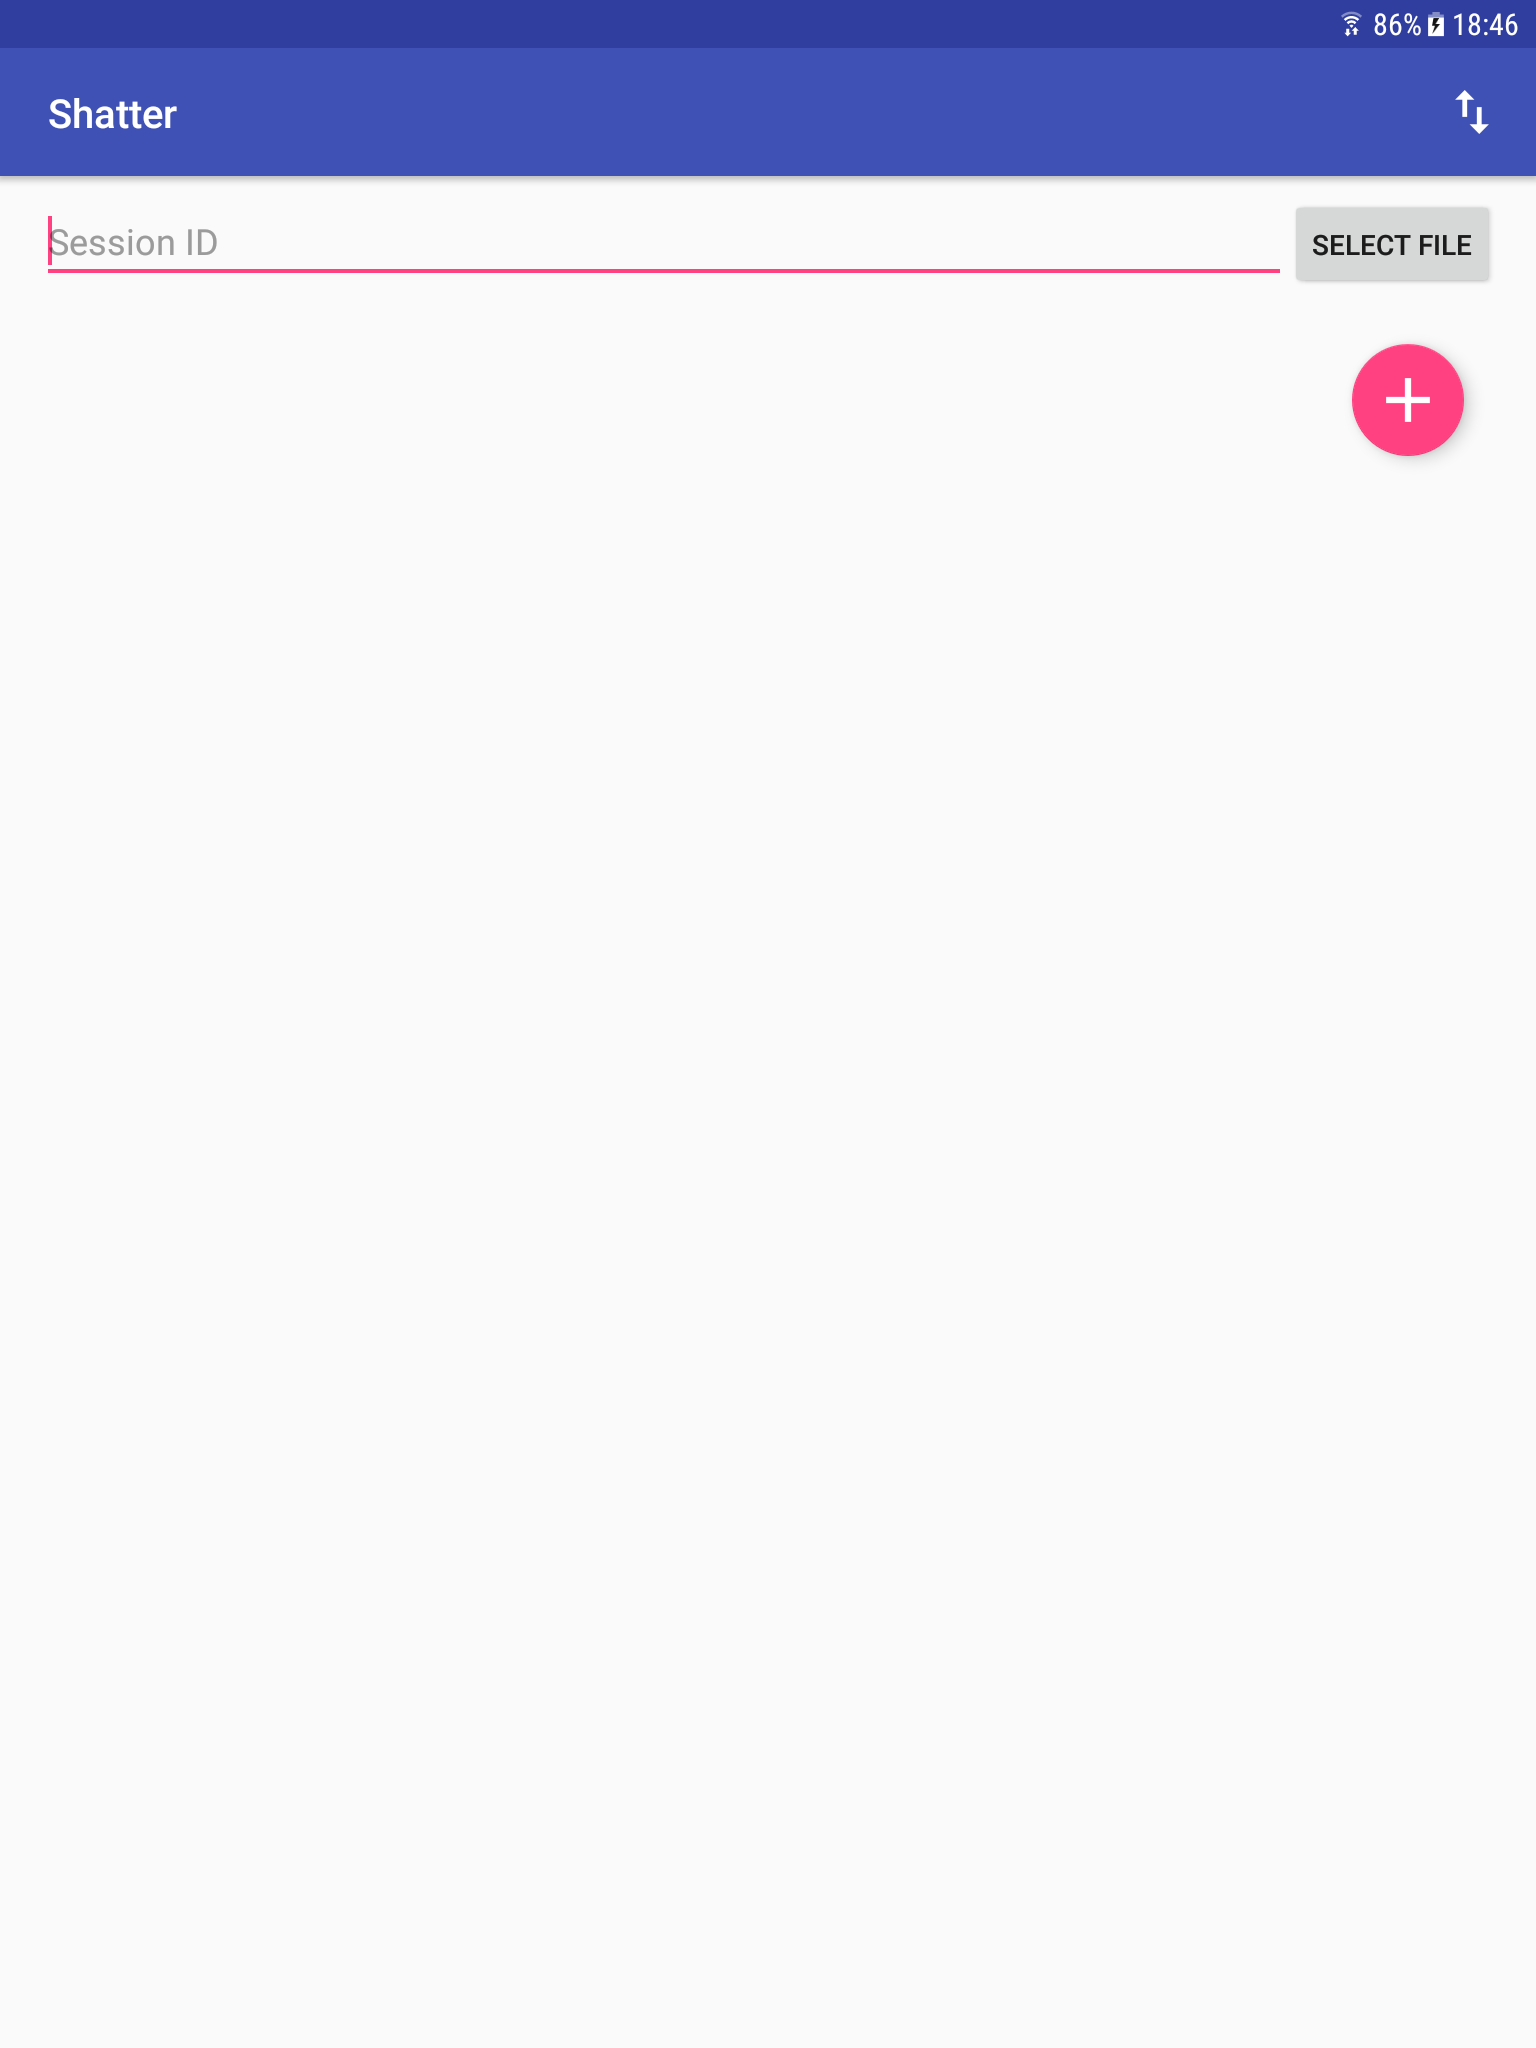
\includegraphics[scale=0.4]{Figures/home}
  \decoRule
  \caption[Shatter (Home)]{Pantalla principal de la aplicación}
  \label{fig:home}
\end{figure}

Como de primeras no disponemos de ningún usuario del que recibir o al que
enviar mensajes, nuestro siguiente objetivo será el de añadir a algún usuario a
nuestra lista de contactos. Lo primero que tendremos que hacer será exportar
nuestra clave pública haciendo uso del icono que se encuentra en la barra
superior de la pantalla principal. (Figura~\ref{fig:export})

\begin{figure}[ht]
  \centering
  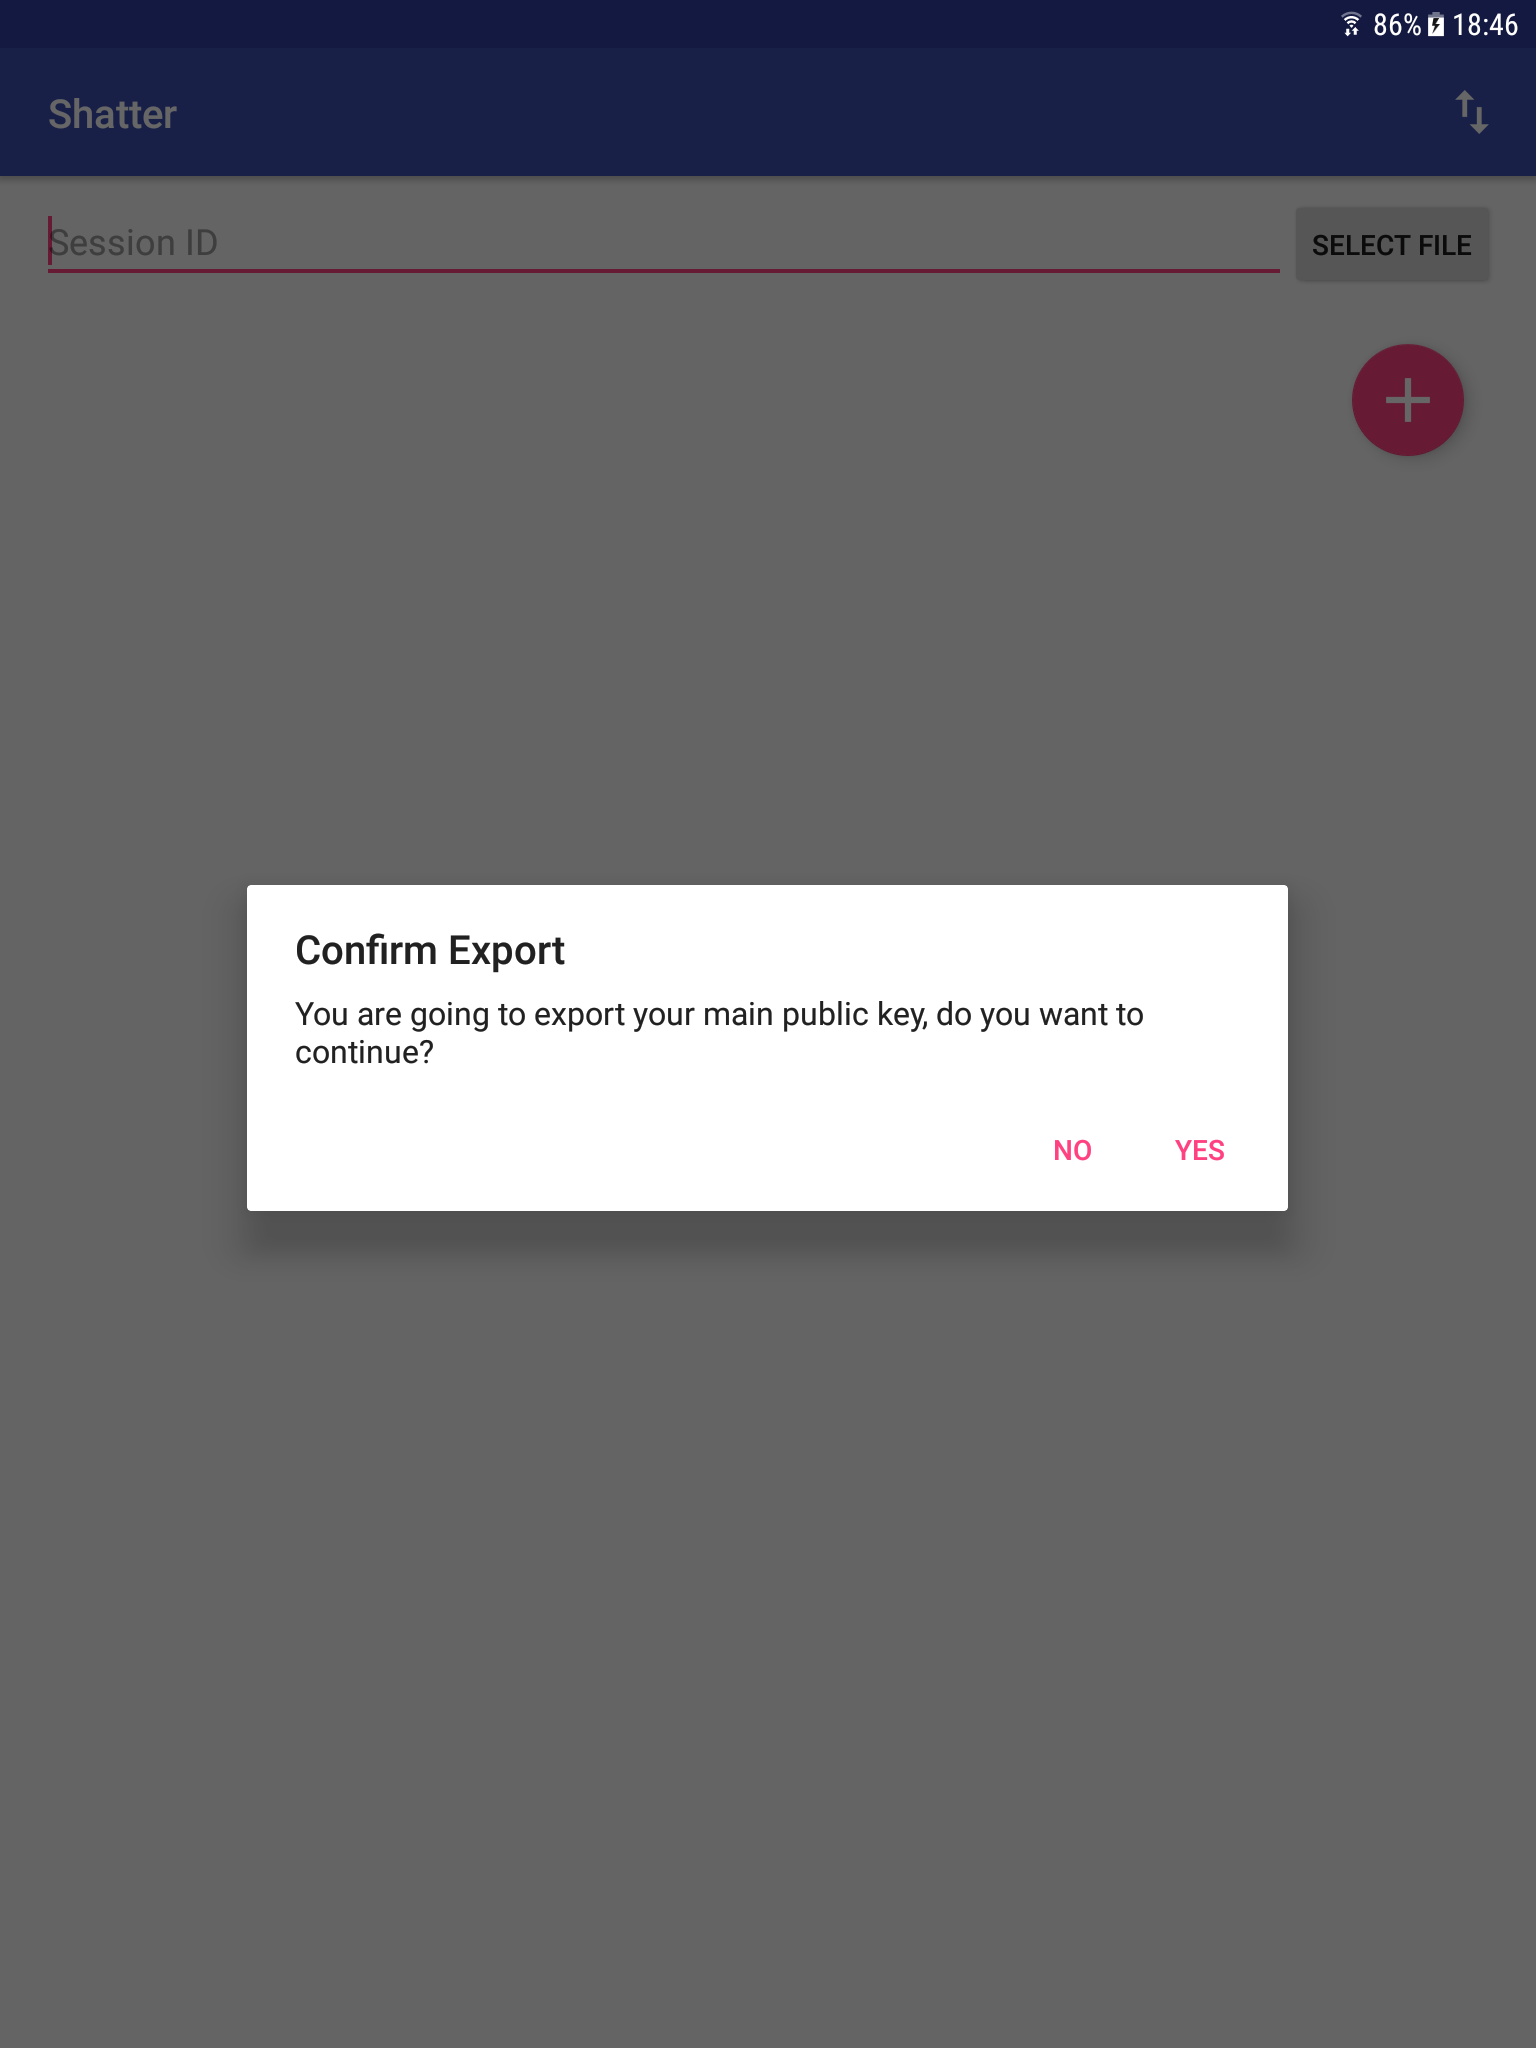
\includegraphics[scale=0.4]{Figures/export}
  \decoRule
  \caption[Shatter (Exportar clave pública)]{Mensaje de advertencia al exportar
  nuestra clave pública}
  \label{fig:export}
\end{figure}

Al confirmar, se habrá generado un certificado el cual contiene nuestra clave
pública en la ruta \path{Shatter/certs/main.crt}. \footnote{El directorio
principal de la aplicación va montado sobre el External Storage del terminal.}

Para añadir a un contacto disponemos de un botón en la esquina inferior derecha
de la pantalla principal, el cual nos abrirá una pantalla nueva en la que
podremos especificar un alias (nombre de usuario) y un certificado con la clave
pública de nuestro amigo. (Figura~\ref{fig:import})

\begin{figure}[ht]
  \centering
  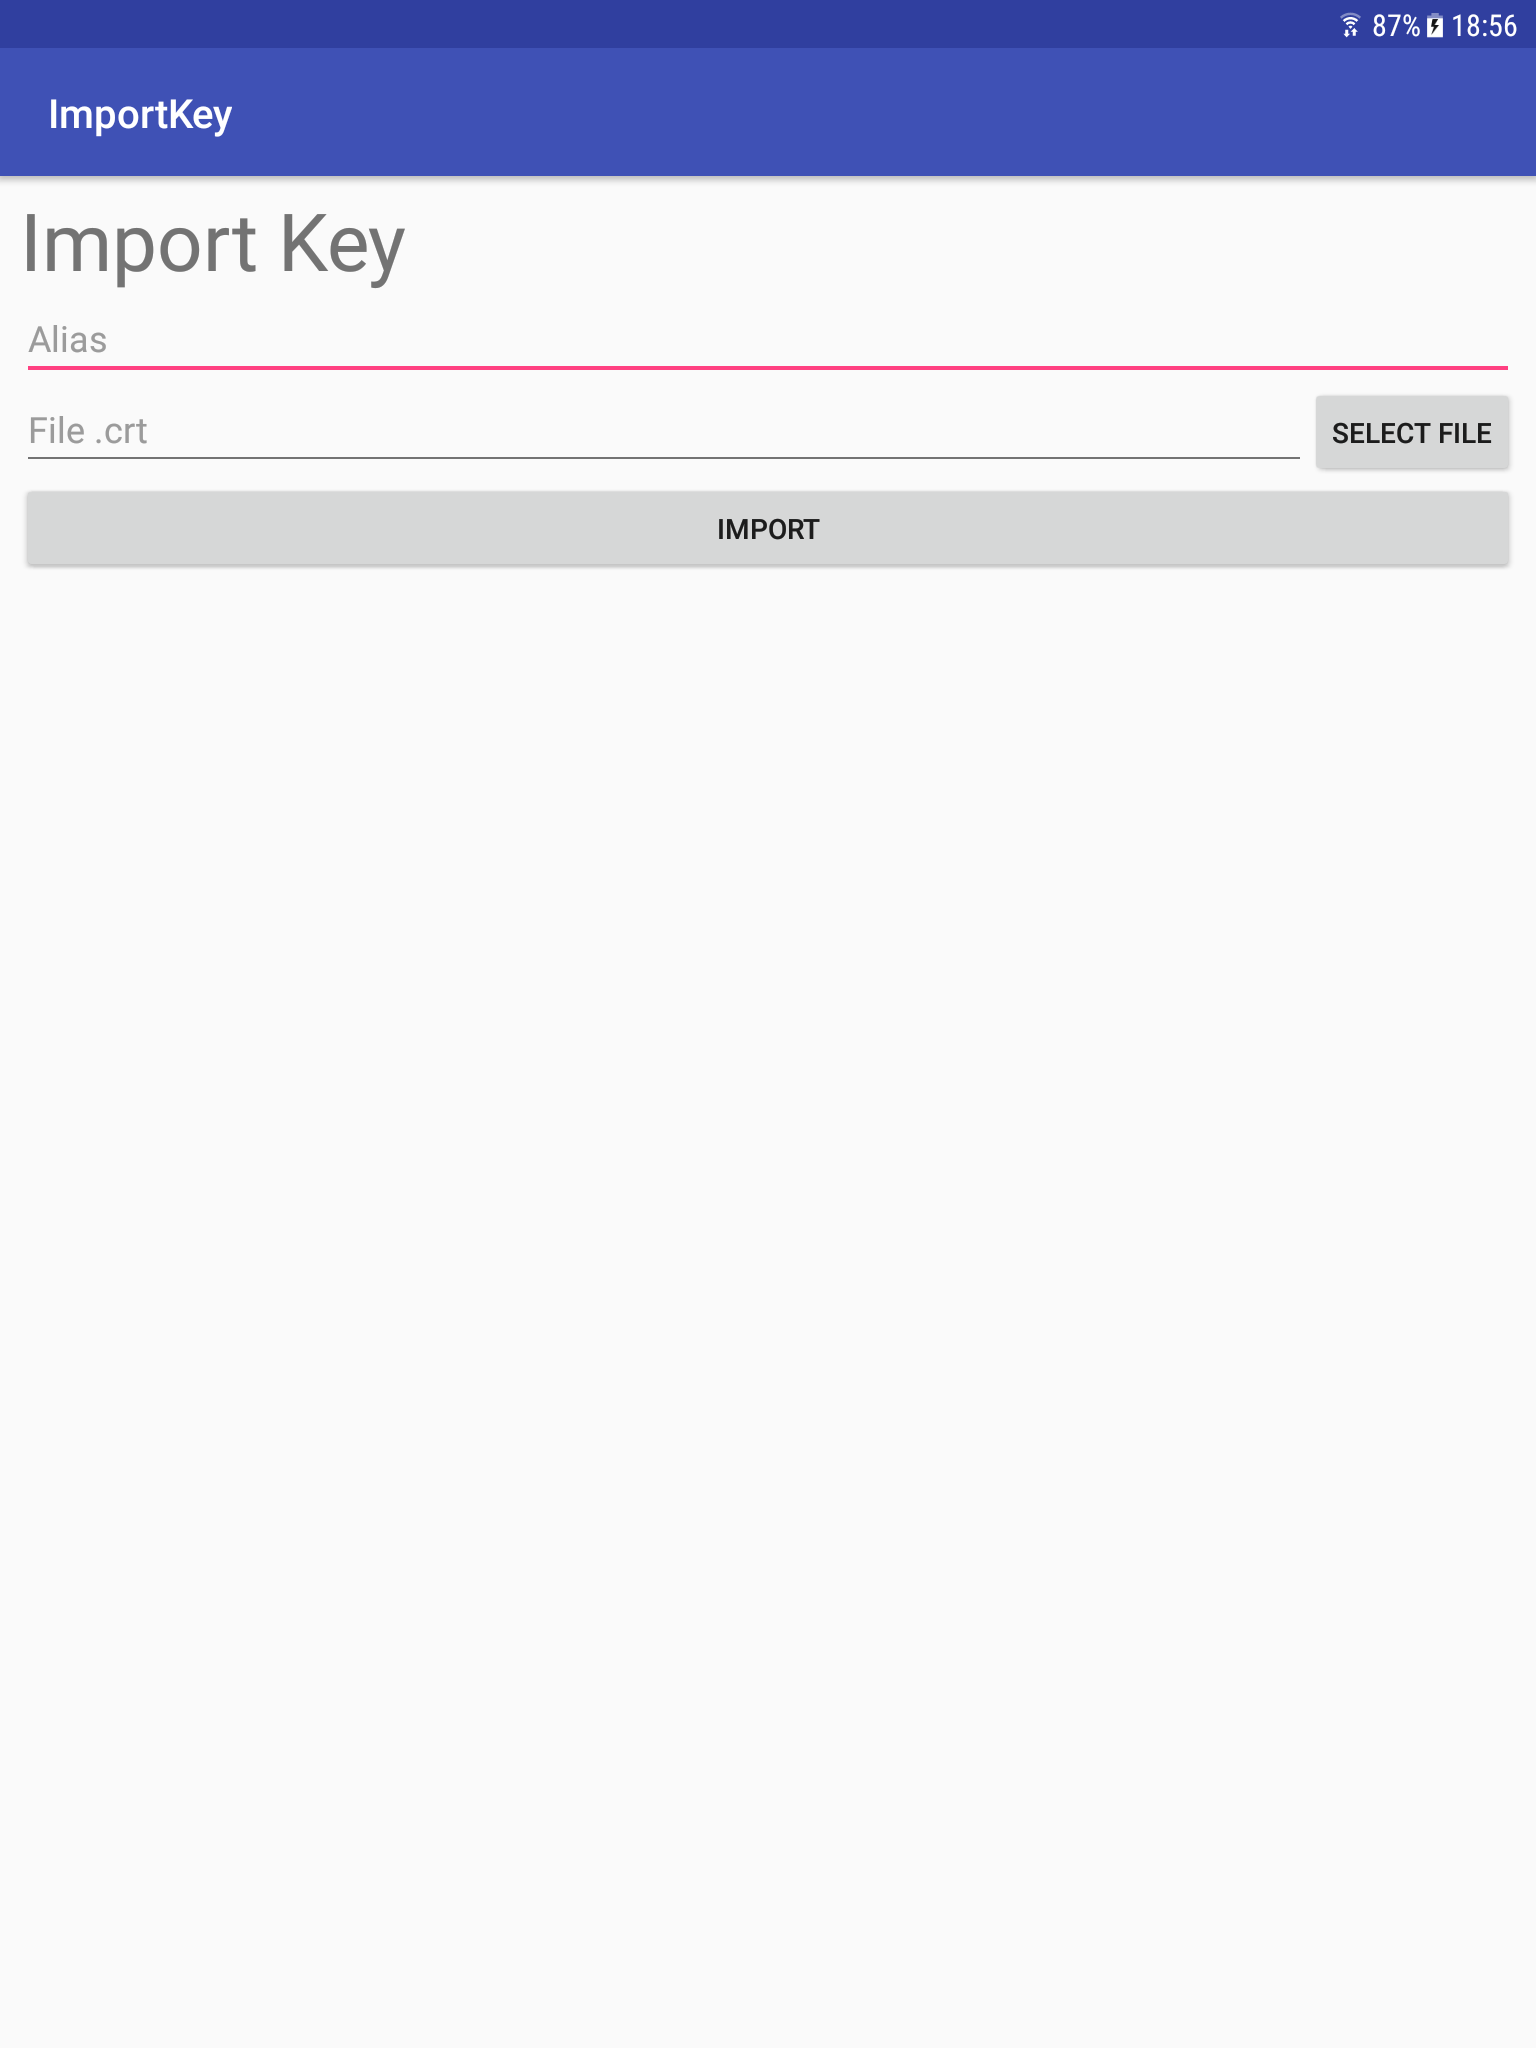
\includegraphics[scale=0.4]{Figures/import}
  \decoRule
  \caption[Shatter (Importar clave pública)]{Pantalla para importar la clave
  pública de un nuevo usuario}
  \label{fig:import}
\end{figure}

Tendremos que compartir nuestra clave pública (previamente generada) con
nuestro nuevo contacto, el cual tendrá que realizar el mismo proceso que hemos
hecho nosotros para importar su clave pública.

Habiendo importado una clave, ésta nos aparecerá en la pantalla principal
representada por su alias para que podamos operar con ella.
(Figura~\ref{fig:home_2})

\begin{figure}[ht]
  \centering
  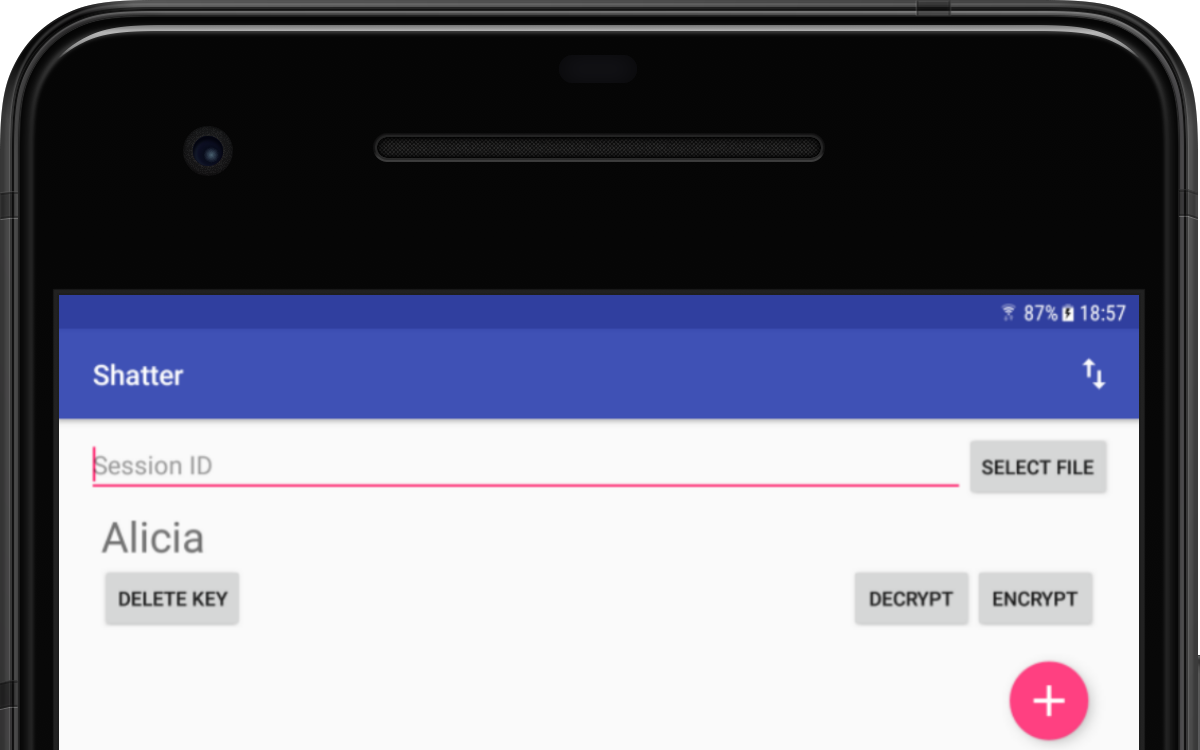
\includegraphics[scale=0.4]{Figures/home_2}
  \decoRule
  \caption[Shatter (Pantalla principal con usuarios)]{Pantalla principal de la
  aplicación con usuarios añadidos}
  \label{fig:home_2}
\end{figure}

Si quisiéramos enviar un mensaje a nuestro nuevo contacto, deberemos utilizar
el botón \emph{Select File}, el cual abrirá una nueva pantalla para que
elijamos el fichero que queramos (Figura~\ref{fig:file_picker}). El selector de
ficheros pondrá en el campo de texto de la pantalla principal el path absoluto
del fichero seleccionado (también podemos escribirlo a mano), y ya solo nos
quedará tocar el botón \emph{Encrypt} del usuario al que vaya destinado el
mensaje para que el fichero se fragmente y encripte. Si todo ha salido bien,
podremos ver un mensaje en pantalla informándonos de ello, y en la ruta
\path{Shatter/send/<ID>} encontraremos los fragmentos junto con la clave.
(Figura~\ref{fig:encfiles})

\begin{figure}[ht]
  \centering
  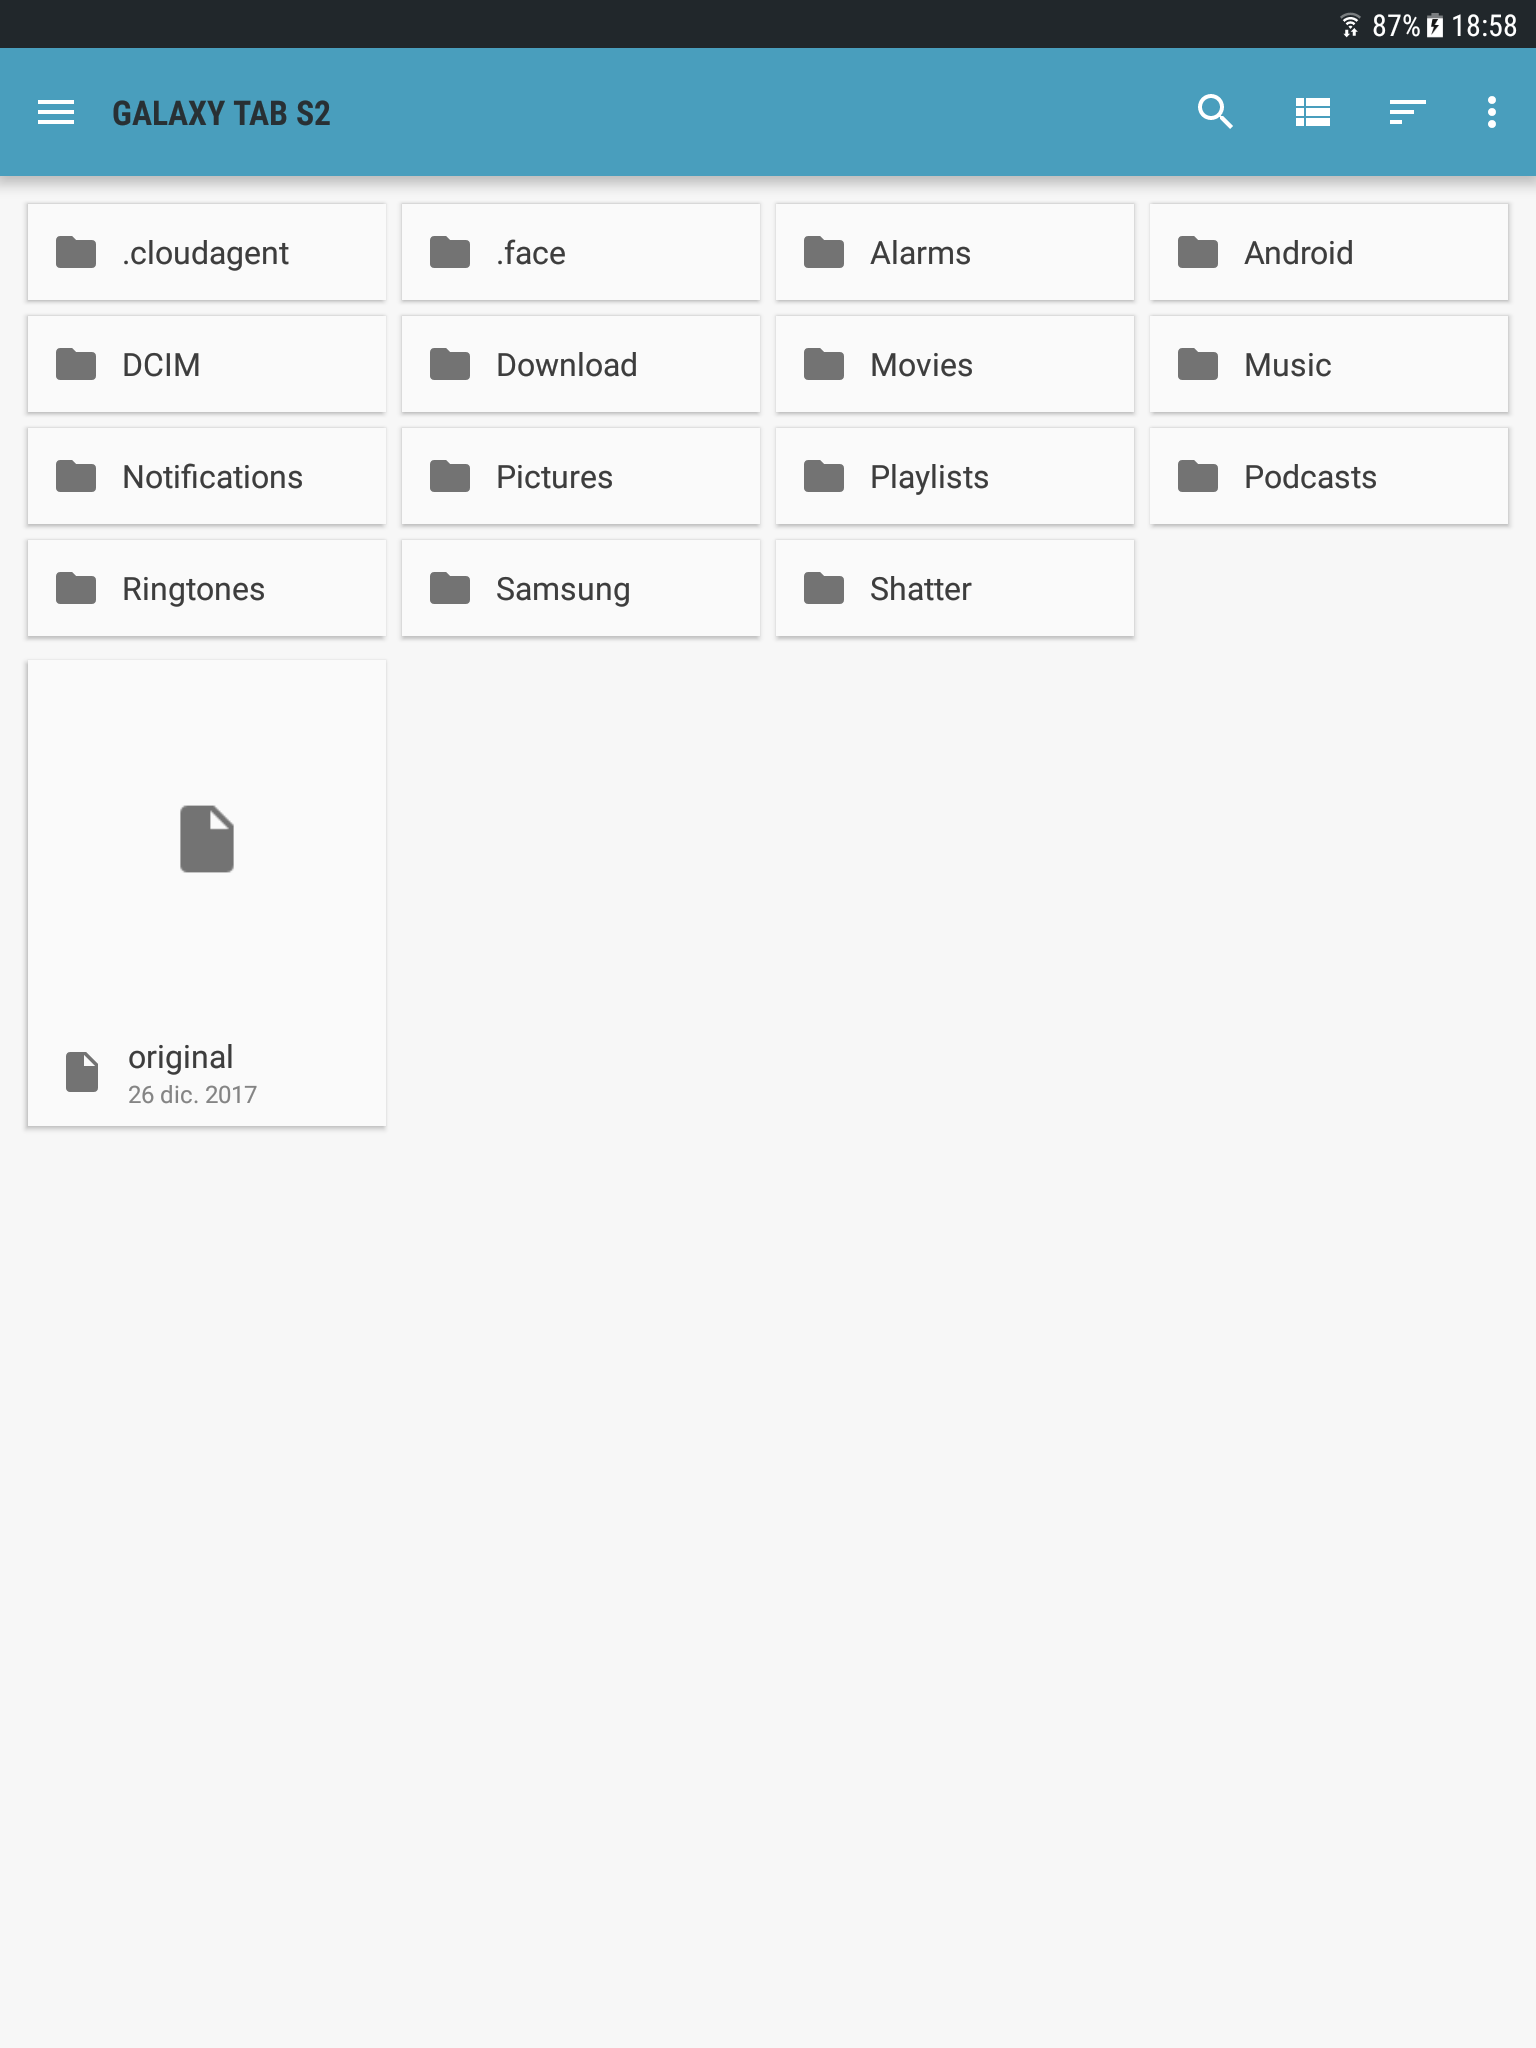
\includegraphics[scale=0.4]{Figures/file_picker}
  \decoRule
  \caption[Shatter (File Picker)]{Pantalla para seleccionar un fichero}
  \label{fig:file_picker}
\end{figure}

\begin{figure}[ht]
  \centering
  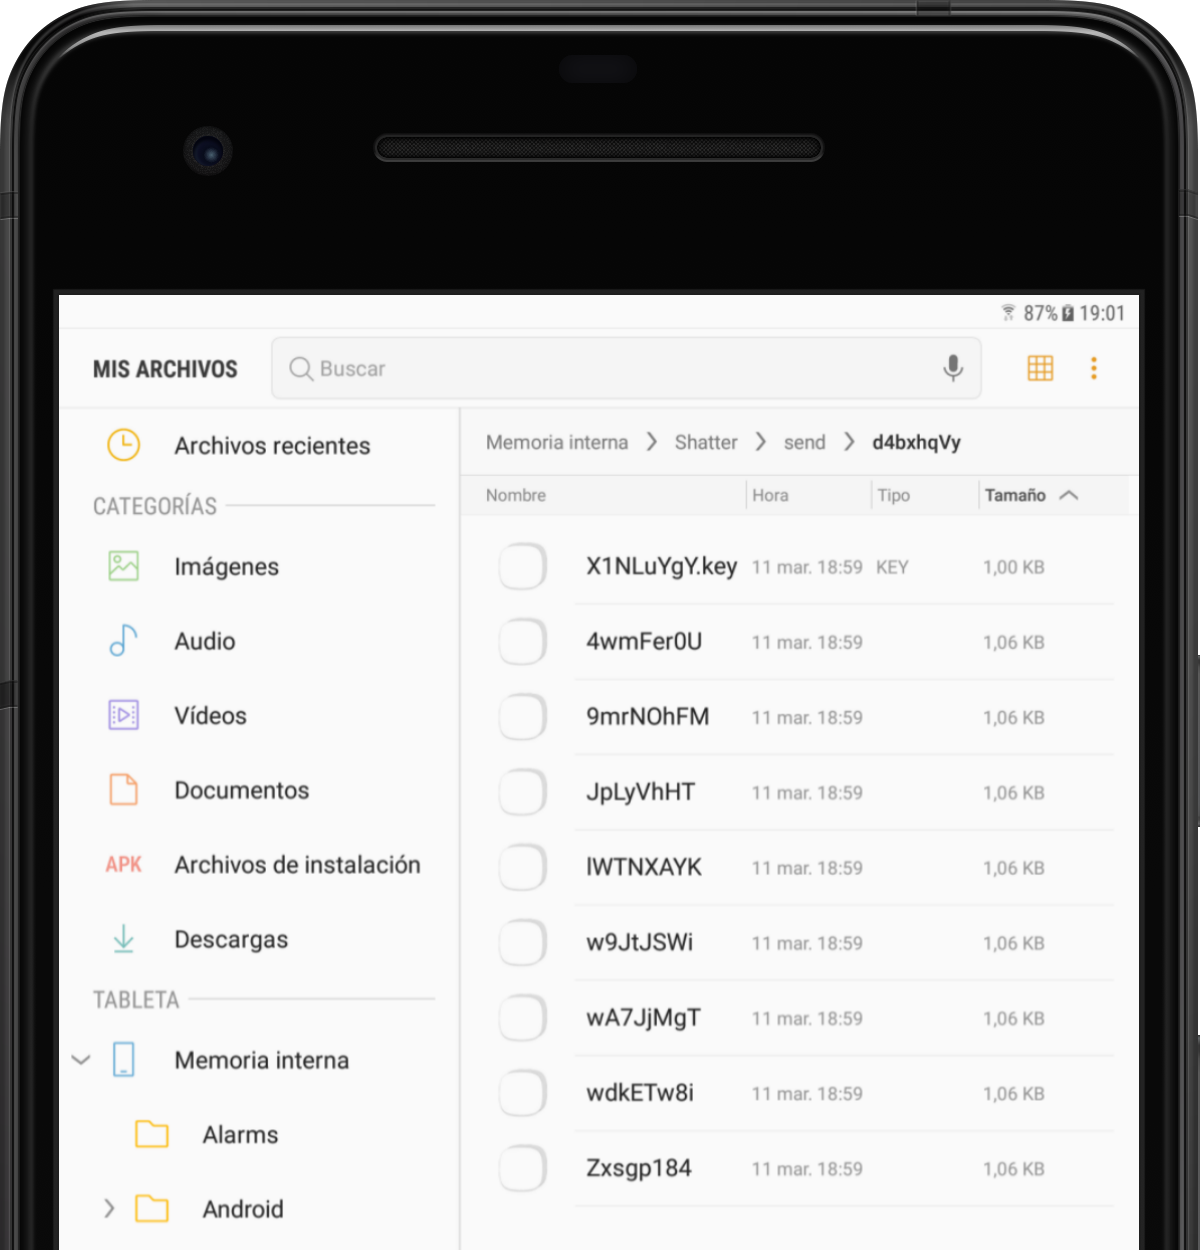
\includegraphics[scale=0.4]{Figures/encfiles}
  \decoRule
  \caption[Shatter (Mensaje fragmentado)]{Fragmentos de un mensaje junto a su
  clave}
  \label{fig:encfiles}
\end{figure}

El ID generado tendremos que comunicárselo al contacto al que vaya destinado,
pero antes deberemos subir el directorio que contiene los fragmentos al servidor
haciendo uso del comando scp de Linux. \footnote{En caso de que estuviéramos
encriptando el mismo mensaje para varios usuarios, podremos saber que ID
corresponde a cada usuario mirando un registro que se encuentra en la ruta
\path{Shatter/list.txt}}

\begin{lstlisting}[language=bash]
  $ scp Shatter/send/<ID> 192.168.1.20:8080
\end{lstlisting}

Si nuestro contacto quisiera descargarse el mensaje, escribirá el ID que le
comunicamos antes en el campo de texto de la pantalla principal. Como sabe que
el mensaje viene de nuestra parte, tocará el botón \emph{Decrypt} de nuestra
clave pública.

La aplicación pedirá al servidor un índice con todos los ficheros asociados a
ese ID y descargará todos los que pueda en el directorio \path{Shatter/<ID>}.
En caso de que algún fichero faltase, informará de ello al usuario antes de
proceder con el descifrado y rellenará un registro indicando cuales son los
fragmentos que faltan. (Figura~\ref{fig:miss})

\begin{figure}[ht]
  \centering
  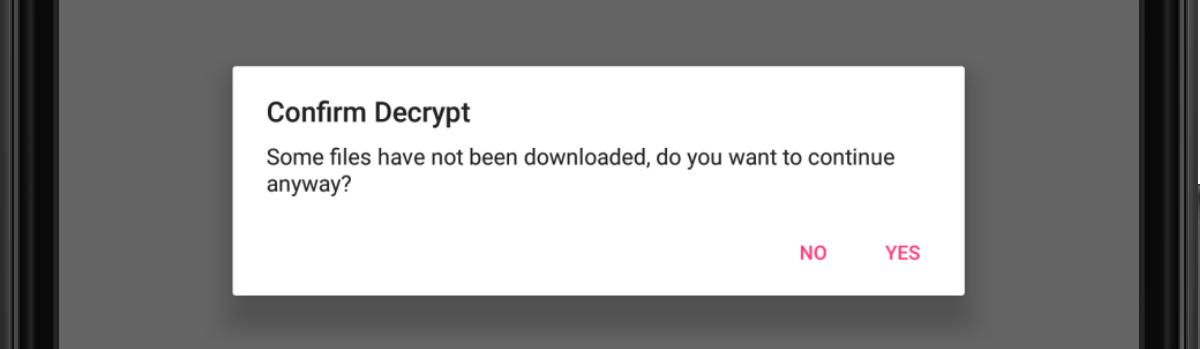
\includegraphics[scale=0.4]{Figures/miss}
  \decoRule
  \caption[Shatter (Faltan fragmentos)]{Mensaje advirtiéndonos de que algunos
  fragmentos no se han descargado}
  \label{fig:miss}
\end{figure}

Si todos los fragmentos y la clave son descargados exitosamente, la aplicación
procederá con el descifrado de los mismos. Durante el proceso se crearán, en
caso de que sea necesario, ficheros de registro en los cuales se reflejará
cualquier problema que haya surgido. En caso de que no ocurra ningún
problema, el fichero original se recompondrá en la ruta
\path{Shatter/<ID>/done/<ID>}. (Figura~\ref{fig:done})

\begin{figure}[ht]
  \centering
  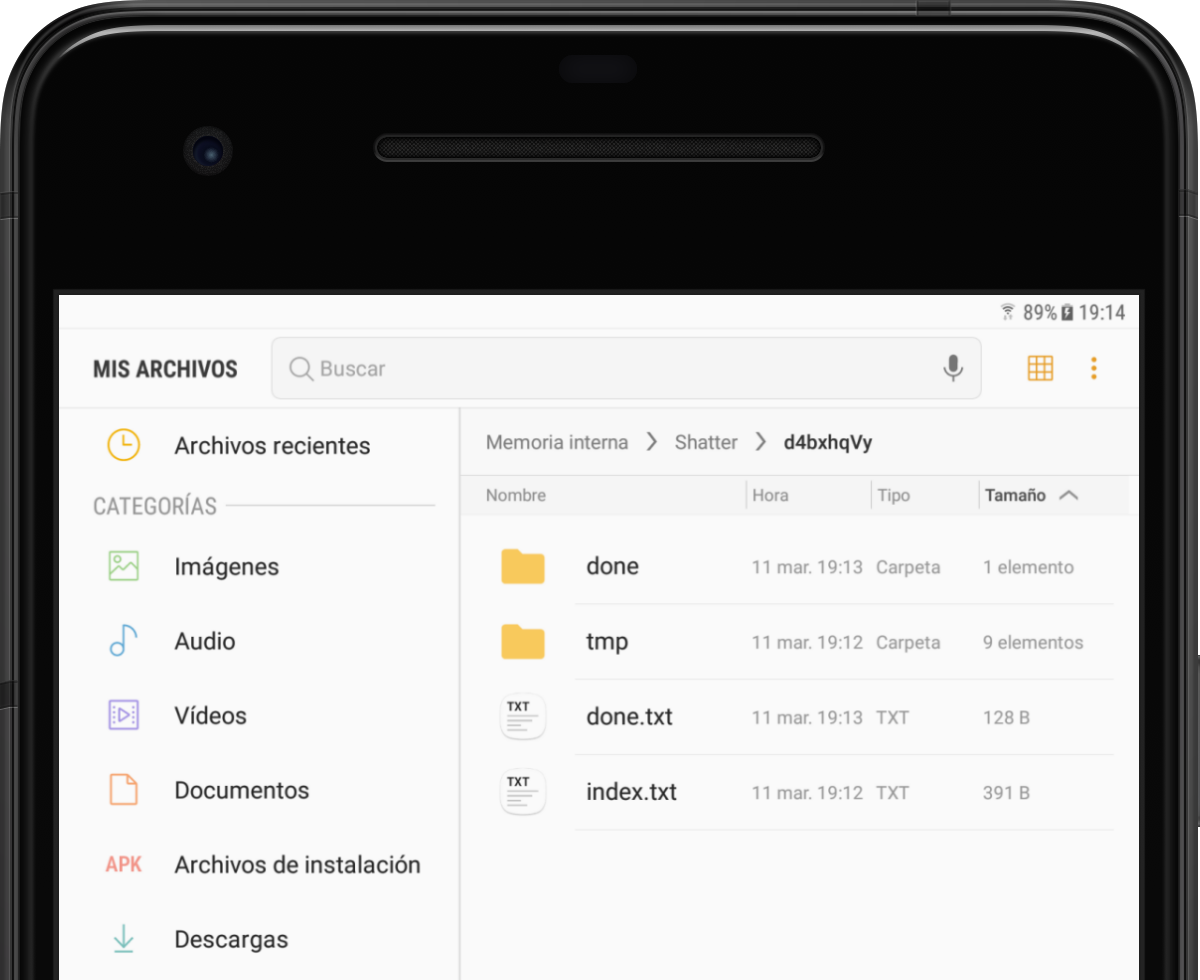
\includegraphics[scale=0.4]{Figures/done}
  \decoRule
  \caption[Shatter (Mensaje recibido)]{Directorio de un mensaje recibido}
  \label{fig:done}
\end{figure}

%----------------------------------------------------------------------------------------

\section{Problemas encontrados}

A lo largo de la etapa que supuso el desarrollo de la aplicación, me encontré
con varios problemas que dificultaron la finalización del proyecto.

El mayor problema con el que se tuvo que lidiar fue el de no haber creado una
parte portable que hiciera más fácil la migración a Android. Algunas librerías
usadas cuando el proyecto solo era una aplicación escrita en Java tenían ciertas
dependencias, las cuales no se encontraban en ninguna librería Java usada en
Android. Además, el uso del KeyStore de Android para almacenar las claves
exigía realizar el cifrado asimétrico, las firmas y la generación de las claves
de una manera determinada, lo que supuso la eliminación de las clases que se
encargaban anteriormente de ello (RSALibrary y RSAPSS). Aunque algunos de estos
problemas no se habrían podido solucionar aun teniendo una parte portable, sin
duda habría supuesto un ahorro considerable de tiempo.

A raíz de lo anterior, la mayoría de las clases no estuvieron bien definidas
desde un principio. Esto supuso muchos cambios a lo largo del desarrollo de la
aplicación (Cabeceras, modos de cifrado, registros...). De nuevo, una buena
planificación habría ahorrado una gran cantidad de tiempo y energía.

Pero no todos los problemas encontrados tuvieron que ver con la desorganización.
La aplicación ahora cuenta con un servidor dedicado pero, en un principio, se
pensó en utilizar un servicio externo para el almacenamiento de los mensajes
enviados por los usuarios. De varias ideas que salieron, se eligió la aplicación
Pastebin\footnote{\url{https://pastebin.com/}}, ya que permite la subida anónima
de texto plano. La idea era que la aplicación subiera los distintos fragmentos
cifrados a la plataforma, permitiendo al resto de usuarios su descarga. Sin
embargo, la existencia de límites en el número de mensajes enviados o en la
longitud de los mismos hicieron que se desechara la idea en favor de un
servidor dedicado.
